\chapter{Methods}

\subsection{Finding the steady states: Newton-Raphson method}

\subsubsection{Newton-Raphson implementation}
To obtain the roots of the system, the Newton-Raphson algorithm was implemented in python using a tolerance value of 0.0001 and a maximum of 15 iterations after which the algorithm stopped searching for a root. Because the system had the potential for multi-stability, several initial conditions need to be searched to obtain all steady states. In total 500 initial conditions were analysed by the Newton-Raphson to obtain all the roots of the system. The 500 conditions were chosen performing latin-hypercube sampling of a 6 dimensional space (6 species) from a uniform distribution with a range from $10^{-3}$ and $10^3$ . Approximately, the root finding for a single parameter set takes around 2 seconds.



\subsection{Linear stability analysis}
%todo look at leyshon paper for lsa explanation

The following section describes how linear stability analysis is carried out for the equilibrium points in a reaction-diffusion system.
The aim of this analysis is to find out if the steady state exhibits a Turing instability or also called a diffusion-driven instability.
When it does, the system is capable of forming spatial patterns.
As the name describes, diffusion-driven instabilities arise in these systems when a homogeneous steady state is stable to small perturbations in the absence of diffusion, and becomes unstable in the presence of diffusion ~\parencite{Glendinning1994, J.DMurray2002}.
To check for Turing instabilities, the stability of the equilibrium state will be studied with and without diffusion.
The method of linear stability analysis will be explained for the two morphogen reaction-diffusion system, shown below:
\begin{subequations}
    \begin{equation}
        \pdv{A}{t} = f_{A}(A,B) + D_{A}\pdv[2]{A}{x}
    \end{equation}
    \begin{equation}
        \pdv{B}{t} = f_{B}(A,B) + D_{B}\pdv[2]{B}{x}
    \end{equation}
\end{subequations}
where $f_{A,B}$ are the non-linear production terms and $D_{A,B}$ are the diffusion constants of the two morphogens.
For future reference, X is a generalisation term to refer to any morphogen A or B.
\subsubsection{Stability of steady state without diffusion}
To study the stability around the steady state without diffusion, Equations 15a and 15b are used, except diffusion terms are removed ($D_{A,B}=0$):
\begin{subequations}
    \begin{equation}
        \pdv{A}{t} = f_{A}(A,B)
    \end{equation}
    \begin{equation}
        \pdv{B}{t} = f_{B}(A,B)
    \end{equation}
\end{subequations}
The steady states are defined as $A^*$ and $B^*$, which satisfy the condition:
\begin{equation}
    f_{A}(A^*,B^*)=0, \hspace{1.5cm} f_{B}(A^*,B^*)=0
\end{equation}
Linear stability analysis is carried by adding an infinitesimally small perturbation $\delta X$ to the steady state $X^*$, and studying if the perturbation decays (stable steady state) or grows (unstable steady state) over time. The perturbation needs to be almost insignificant as Taylor expansion is carried out to linearise the system around the steady state. Therefore, the morphogen concentration can be expressed as:
\begin{subequations}
    \begin{equation}
        A(t) = A^* + \delta A(t),\hspace{1.5cm} |\delta A| <<A^*
    \end{equation}
    \begin{equation}
        B(t) = B^* + \delta B(t), \hspace{1.5cm} |\delta B| <<B^*
    \end{equation}
\end{subequations}
The differential equations 16a and 16b are re-evaluated, using equations 17 and 18a,b:
\begin{subequations}
    \begin{equation}
        \pdv{A}{t} = \pdv{[A^* + \delta A(t)]}{t} = f_{A}(A^* + \delta A(t), B^* + \delta B(t)) = \pdv{\delta A}{t}
    \end{equation}
    \begin{equation}
        \pdv{B}{t} = \pdv{[B^* + \delta B(t)]}{t} = f_{B}(A^* + \delta A(t), B^* + \delta B(t)) = \pdv{\delta B}{t}
    \end{equation}
\end{subequations}
As previously mentioned, the non-linear system will be linearised around the steady state using Taylor expansion.
This is done to have a simpler set of equations, that represent the system around the steady state, as seen below:
\begin{equation}
    f(A+\delta A, B+\delta B) = f(A,B) + \pdv{f(A,B)}{A}\delta A + \pdv{f(A,B)}{B}\delta B + ... + \frac{1}{n!} \pdv[n]{f(A,B)}{A}\delta A^n + \frac{1}{n!} \pdv[n]{f(A,B)}{B}\delta B^n
\end{equation}
If $\delta A$ and $\delta B$ are small enough, higher order terms can be ignored as $\delta (A,B)^n$  becomes infinitesimally small.
Furthermore, it can be assumed that $f(A^*,B^*) = 0$, therefore the following expression is obtained, where $f$ corresponds to either $f_{A}$ or $f_{B}$  :
\begin{equation}
    f(A^*+\delta A, B^*+\delta B) =  \pdv{f(A,B)}{A}\delta A + \pdv{f(A,B)}{B}\delta B
\end{equation}
Finally, because $\pdv{X}{t} =  \pdv{\delta X}{t}$ (as seen in Equations 19a and 19b), the change in perturbation (decay or growth) can be expressed as:
\begin{subequations}
    \begin{equation}
        \pdv{\delta A}{t} = \pdv{f_{A}(A,B)}{A}\delta A + \pdv{f_{A}(A,B)}{B}\delta B
    \end{equation}
    \begin{equation}
        \pdv{\delta B}{t} = \pdv{f_{B}(A,B)}{A}\delta A + \pdv{f_{B}(A,B)}{B}\delta B
    \end{equation}
\end{subequations}
The general solution can be expressed as an exponential, where $\sigma$ determines the growth rate of the perturbation, and whether it grows (unstable steady state) or decays (stable steady state):
\begin{subequations}
    \begin{equation}
        \delta A = A_{0}e^{\sigma t}
    \end{equation}
    \begin{equation}
        \delta B = B_{0}e^{\sigma t}
    \end{equation}
\end{subequations}
If Equations 23a and 23b are introduced into 22a and 22b, and the solution divided by $e^{\sigma t}$ on both sides, the following is obtained:
\begin{subequations}
    \begin{equation}
        \sigma \delta A_{0} = \pdv{f_{A}(A,B)}{A} \delta A_{0} + \pdv{f_{A}(A,B)}{B}\delta B_{0}
    \end{equation}
    \begin{equation}
        \sigma \delta B_{0} = \pdv{f_{B}(A,B)}{A} \delta A_{0}+ \pdv{f_{B}(A,B)}{B}\delta B_{0}
    \end{equation}
\end{subequations}
This can be represented as an eigenvalue-eigenvector problem using the jacobian $\textbf{J}$, the eigenvalue $\sigma$ and the eigenvector  $\delta u_{X} = [u_{A},u_{B}]$:
\begin{equation}
    \sigma \delta X_{0} = \begin{bmatrix}
                              \pdv{f_{A}}{A} &
                              \pdv{f_{A}}{B}  \\
                              \pdv{f_{B}}{A} &
                              \pdv{f_{B}}{B}
    \end{bmatrix}\delta X_{0}
\end{equation}
Finally, $\sigma$ can be obtained by solving:
\begin{equation}
    p(\sigma) = det[J-\sigma I] = 0
\end{equation}
The real part of $\sigma$ corresponds to the growth rate of the perturbation (Equations 23a and 23b). $Im(\sigma)$ corresponds to the oscillations, which can be ignored for now. If $Re(\sigma) < 0 $, the steady state will be stable to perturbations, which means the system will go back to steady state after a small perturbation is applied. If $Re(\sigma) > 0 $, the steady state will be unstable to perturbations, and the system will go away from the equilibrium point after being slightly perturbed.
\subsubsection{Stability of steady state with diffusion}
Once the stability of the steady state has been analysed in the absence of diffusion, the effect of diffusion on the same system will be studied. The diffusion will be introduced through the partial derivative term $D_{X}\pdv[2]{[X]}{x}$, where X is the morphogen, giving rise to Equations 15a and 15b.
\paragraph{Reduction of PDE term to ODE through Fourier transformations}
The second order partial derivative term will be reduced to an ODE simpler term through Fourier transforms. For this purpose, the following Fourier transform definitions are used:
\begin{subequations}
    \begin{equation}
        F(k) = \mathcal{F}(f(x)) = \int_{-\infty}^{\infty} f(x)e^{-ikx} dx
    \end{equation}
    \begin{equation}
        f(x) = \mathcal{F}^{-1}(F(k)) = \frac{1}{2\pi}\int_{-\infty}^{\infty} F(k)e^{ikx} dk
    \end{equation}
\end{subequations}
First, using the inverse Fourier transform (Equation 27b), the first order partial derivative will be reduced to an ODE form:
\begin{equation}
    \begin{split}
        \pdv{[X(x,t)]}{x}) = \mathcal{F}^{-1}\left(\pdv{[X(k,t)]}{x}\right) = \pdv{}{x}\left[\frac{1}{2\pi}\int_{-\infty}^{\infty} X(k,t)e^{ikx} dk\right] =  \frac{1}{2\pi}\int_{-\infty}^{\infty} X(k,t)\frac{d}{dx}e^{ikx} dk\\\\ =\frac{1}{2\pi}\int_{-\infty}^{\infty} ik X(k,t)e^{ikx} dk = ik \frac{1}{2\pi}\int_{-\infty}^{\infty} X(k,t)e^{ikx} dk = ik X(x,t)
    \end{split}
\end{equation}
giving $\pdv{[X(x,t)]}{x}) =  ik X(x,t)$.
Using this expression, the inverse Fourier transform (Equation 22b) and the fact that $\pdv[2]{X(x,t)}{x} =\left(\pdv{X(x,t)}{x}\right)^2$, the following expression is obtained:
\begin{equation}
    \begin{split}
        \pdv[2]{[X(x,t)]}{x}) = \left(\pdv{X(x,t)}{x}\right)^2 = \mathcal{F}^{-1}\left[\pdv{[ikX(k,t)]}{x}\right] = \pdv{}{x}\left[\frac{1}{2\pi}\int_{-\infty}^{\infty} ikX(k,t)e^{ikx} dk\right] \\\\=  \frac{1}{2\pi}\int_{-\infty}^{\infty} ikX(k,t)\frac{d}{dx}e^{ikx} dk =\frac{1}{2\pi}\int_{-\infty}^{\infty} (ik)^2 X(k,t)e^{ikx} dk = -k^2 \frac{1}{2\pi}\int_{-\infty}^{\infty} X(k,t)e^{ikx} dk = -k^2 X(x,t)
    \end{split}
\end{equation}
giving
\begin{subequations}
    \begin{equation}
        \pdv[2]{A(x,t)}{x} = -k^2\cdot A
    \end{equation}
    \begin{equation}
        \pdv[2]{B(x,t)}{x} = -k^2\cdot B
    \end{equation}
\end{subequations}
This way, the second order partial derivative terms, are reduced to simpler ODE systems to be used in linear stability analysis
\paragraph{Definition of boundary conditions}
The system is defined within some boundaries, meaning x goes from 0 to L. In this case, no molecules can leave the system, so the boundary condition applied is a zero-flux boundary condition. At the boundaries, the partial derivative is zero, defined below as Neumann Boundary conditions:
\begin{equation}
    \pdv[2]{X(x=0,t)}{x}=0  \hspace{0.5cm}\And  \hspace{0.5cm}\pdv[2]{X(x=L,t)}{x}=0
\end{equation}
This can be visualised as a fish tank, of length L, filled with water: water diffuses freely within the tank, but cannot diffuse outside the boundaries. In addition, the levels of water at the boundaries are not fixed. For the spatial derivatives to be zero at the boundaries, some restrictions will need to be applied. The expression from Equation 29 will be used to apply our boundary conditions.
\begin{equation}
    \begin{split}
        \pdv[2]{[X(x,t)]}{x}) =  -k^2 \frac{1}{2\pi}\int_{0}^{L} X(k,t)e^{ikx} dk =  -k^2 \frac{1}{2\pi}\int_{0}^{L} X(k,t)(cos(kx)+isin(kx))dk\\\\
        =\frac{-k^2}{2\pi}\left(\int_{0}^{L} X(k,t)cos(kx)dk + i\int_{0}^{L} X(k,t)sin(kx)dk\right)
    \end{split}
\end{equation}
The first integral is integrated by parts to express the equation in terms of $sin(kx)$:
\begin{equation}
    \begin{split}
        \pdv[2]{[X(x,t)]}{x}) = \frac{-k^2}{2\pi}\left(\left[\frac{sin(kx)}{k}X(k,t)\right]^L_{0} - \int_{0}^{L} \frac{sin(kx)}{k}\pdv{A(k,t)}{k}dk + i\int_{0}^{L} X(k,t)sin(kx)dk\right)
    \end{split}
\end{equation}
As defined with the boundary conditions (Equation 31), the partial derivative must be 0 at $x=0$ and  $x=L$. Therefore, at $x=0$ and  $x=L$, $sin(kx)=0$. For the two boundary conditions:
\begin{itemize}
    \item When $x=0$: $sin(k\cdot0)=sin(0)=0$. Therefore for $x=0,\pdv[2]{X(0,t)}{x}=0$.
    \item When $x=L$: $sin(k\cdot L)$ must be zero. If $ k=\frac{n\pi}{L}$, $sin(kL) = sin(n\pi) = 0$. Therefore, for $x=L$ , $\pdv[2]{X(L,t)}{x}=0 \hspace{0.5cm} \forall n \in \{0, \mathbb{N}\} $
\end{itemize}
Following these calculations, the zero-flux boundary condition is applied when $k=\frac{n\pi}{L} \hspace{0.1cm}\forall n \in \{0, \mathbb{N}\} $

\paragraph{Linear Stability Analysis of steady state with diffusion effects}
Now that the PDE diffusion term has been reduced to an ODE term, and the zero-flux boundary conditions introduced, the stability of the steady state when introducing diffusion can be studied.
As shown in Equations 30a and 30b, the diffusion term $D_{X}\pdv[2]{X}{x} $ can be expressed as $-k^2X$, therefore the reaction-diffusion PDE equations are reduced to:
\begin{subequations}
    \begin{equation}
        \pdv{A}{t} = f_{A}(A,B)  -k^2A
    \end{equation}
    \begin{equation}
        \pdv{B}{t} = f_{B}(A,B) -k^2B
    \end{equation}
\end{subequations}
where $k=\frac{n\pi}{L} \hspace{0.1cm}\forall n \in \{0, \mathbb{N}\} $.
In the previous section, the linear stability analysis was carried around the steady state with a perturbation $\delta X$ (diffusion not included). Using Equation 21, which describes the linearised reaction terms around the steady state, Equations 34 can be expressed as:


\begin{subequations}
    \begin{equation}
        \pdv{\delta A}{t} = \pdv{f_{A}(A,B)}{A}\delta A + \pdv{f_{A}(A,B)}{B}\delta B  -D_{A}k^2\delta A
    \end{equation}
    \begin{equation}
        \pdv{\delta B}{t} =  \pdv{f_{B}(A,B)}{A}\delta A + \pdv{f_{B}(A,B)}{B}\delta B  -D_{B}k^2\delta B
    \end{equation}
\end{subequations}

The general solution of this system can be written as:

\begin{subequations}
    \begin{equation}
        \delta A = A_{0}e^{\sigma t}\cdot e^{ikx}
    \end{equation}
    \begin{equation}
        \delta B = B_{0}e^{\sigma t}\cdot e^{ikx}
    \end{equation}
\end{subequations}
where $X_{0}e^{\sigma t}$ represents the amplitude of the perturbations and $e^{ikx}$ represents the spatial oscillations (with $k$ as the wavenumber). In this case, we are interested on the growth or decay of the perturbations over time. Therefore, to observe the stability of the steady state, we will study the amplitude term ($X_{0}e^{\sigma t}$):
\begin{itemize}
    \item If $\sigma > 0$: perturbation ($\delta X$) grows making $\pdv{\delta A}{t} > 0$. Therefore, the steady state is unstable with diffusion.
    \item If $\sigma < 0$: perturbation ($\delta X$) decays making $\pdv{\delta A}{t} < 0$. Therefore, the steady state is stable with diffusion.
\end{itemize}
If Equations 36a and 36b are substituted into Equations 35a and 35b, the following equations are obtained:
\begin{subequations}
    \begin{equation}
        \sigma \delta A_{0} = \pdv{f_{A}(A,B)}{A} \delta  A_{0}  + \pdv{f_{A}(A,B)}{B}\delta  B_{0} -D_{A}k^2\delta  A_{0}
    \end{equation}
    \begin{equation}
        \sigma \delta B_{0}= \pdv{f_{B}(A,B)}{A} \delta  A_{0}  + \pdv{f_{B}(A,B)}{B}\delta  B_{0}  -D_{B}k^2\delta A
    \end{equation}
\end{subequations}
These pair of equations can again be treated as an eigenvalue-eigenvector problem written in the following way:
\begin{equation}
    \sigma \delta X_{0} = \begin{bmatrix}
                              \pdv{f_{A}}{A} - D_{A}k &
                              \pdv{f_{A}}{B}  \\
                              \pdv{f_{B}}{A} &
                              \pdv{f_{B}}{B} - D_{B}k
    \end{bmatrix}\delta X_{0}
\end{equation}
where $\sigma$ can be solving the characteristic polynomial:
\begin{equation}
    p(\sigma) = det[J-\sigma I] = 0
\end{equation}
In summary, to understand if perturbations around the steady state decay or grow when diffusion is introduced, Equation 39 must be solved to obtain $\sigma$. This characteristic polynomial is solved for a range of k's, being $k=\frac{n\pi}{L} \hspace{0.1cm}\forall n \in \{0, \mathbb{N}\} $. The sign of $\sigma$ is studied for every k, resulting in the dispersion relation (Figure 2 in the Introduction). If $\sigma > 0$, perturbations grow around the steady state and the system is unstable. In the contrary, if  $\sigma < 0$, the system is stable and perturbations decay around the steady state. More detail on linear stability analysis can be found in \cite{J.DMurray2002} or \cite{Glendinning1994}.
\subsubsection{Linear stability analysis implementation}
Linear stability analysis is carried out with and without diffusion for all steady states of the system found using Newton-Raphson. The analysis is done for all $k=\frac{n\pi}{L} \hspace{0.1cm}\forall \{n \in \mathbb{N} : n \leq 5000\} $, meaning 5000 k's are sampled using linear stability analysis. L is defined as 100mm.  Linear stability analysis for a single steady state takes approximately approximately 1 second.

\subsection{Sampling method}
If no parameters from a system are known, sampling of the whole parameter space must be done to understand the systems behaviour. Different methods exist for sampling parameter spaces. Several studies have shown that latin-hypercube sampling (LHS) has a higher efficiency than grid sampling or random sampling when searching through high dimensional spaces. The efficiency over grid sampling might be explained because not all dimensions of the model are important, meaning some parameters might be sloppy. Therefore not all parameters have to be explored thoroughly as done in grid sampling \parencite{iman1980latin, Bergstra2012}. The three sampling regimes are shown in Figure 20a.\\\\
In LHS, a distribution and a number of desired samples is given as an input. The algorithm then divides the space sections according to the distribution given (e.g in a normal distribution, more sections will appear near the mean value).  Then, one sample is positioned randomly somewhere in each section. For a 2 dimensional parameter space, no samples can be in the same column or row. This is scaled up to high multidimensional spaces such as the 22 dimensional space of the model proposed. This scheme is shown in Figure 20b.
%\begin{figure}[H]
%    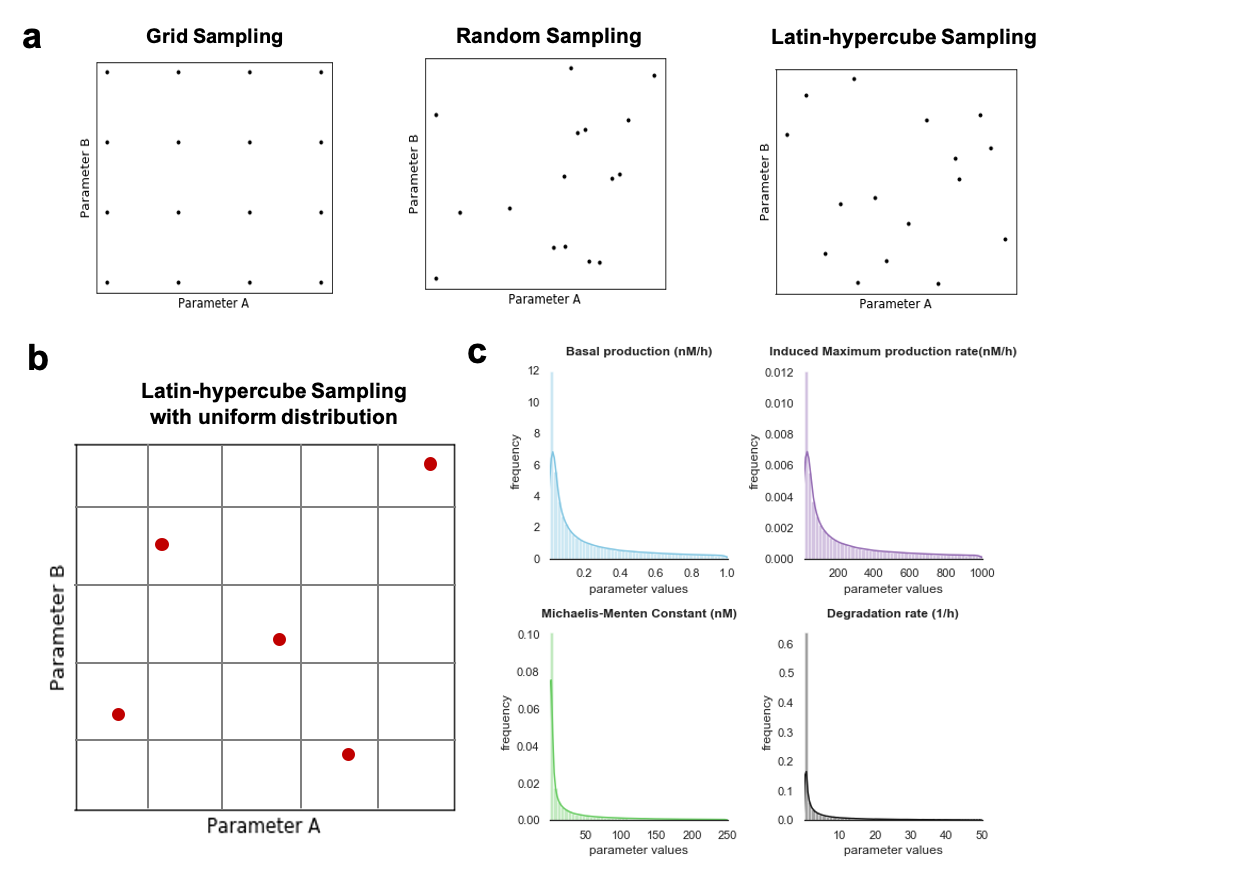
\includegraphics[width=1.1\textwidth]{Methods/sampling.png}
%    \caption{\textbf{Sampling method for high dimensional spaces}. \textbf{(A)} Types of potential sampling methods. \textbf{(B)} Latin-Hypercube sampling with uniform distribution for a 2 dimensional parameter space. Space is separated in 5 sections for each parameter, leading to 5 samples (red dot). No sample is present in the same row or column. \textbf{(C)} Parameter distributions used for Latin-hypersube sampling. The 4 different types of parameters have different distributions depending on the ranges defined. All of them are uniform distributions in log-scale. }
%\end{figure}
The distribution given as an input to the LHS algorithm, will be the resulting distribution of your samples. For the purpose of this search, the distributions chosen are uniform distributions in a logarithmic scale (log-uniform distribution). The uniform distribution, although it does not describe many phenomena in biology, can be useful when no prior knowledge is known about the parameters \parencite{Frank2009TheNature}. The logarithmic component is used to make sure parameters from all scales are represented equally, instead of having a higher frequency of values from larger scales. Log-normal distributions are commonly used for modelling in biology, however due to the nonexistent prior knowledge on our parameter values, the log-uniform is used instead. The log-uniform distribution is defined within a certain range, which varies depending on the parameter type. The distributions for each parameter type are shown in Figure 20c. Overall, 1 million samples where produced using the LHS with a uniform distribution in log-scale. All parameters except the diffusion rates ($d$) and the cooperativity ($n$) where sampled using LHS and the distributions shown in Figure 20c.


\subsection{Numerical solution by finite-difference methods}
Obtaining a solution for a system of equations can become a complex problem if working with a system of 6 non-linear PDEs. Because an analytical expression for the solution is almost impossible to obtain, finite-difference methods are used for cases like this one. Finite-difference methods consists in discretising space and time to approximate the PDE system to a system of algebraic equations that can be easily solved by matrix algebra techniques \parencite{morton2005numerical}. By discretising time and space, the two independent variables can be expressed as:
\begin{subequations}
    \begin{equation}
        t_{n} = n\Delta t, n=0,...,N-1
    \end{equation}
    \begin{equation}
        x_{j} = j\Delta x, j=0,...,J-1
    \end{equation}
\end{subequations}
While $\Delta t$ and $\Delta x$ are the time steps and the space steps respectively, N and J are the number of discrete time and space points in our grid. $\Delta t$ and $\Delta x$ can be defined as $ \Delta t = \frac{T}{N}$ and $   \Delta x= \frac{L}{J}$ respectively where T and L are the final time and space values in the grid. The aim is to derive a numerical solution that is approximates to the unknown analytical solution so $U(j\Delta x, n\Delta t)\approx u( j\Delta x, n\Delta t)$, where $U$ is the analytical solution and $u$ is the numerical solution. \\\\
When working with a numerical solver, the solver can perturb the systems behaviour due to the effects of the time-step, the integration method or the computer arithmetic. When choosing a scheme to numerically solve a PDE, three different characteristics of the scheme need to be considered: Consistency, stability and convergence. Firstly, for a scheme to be consistent, the truncation error must be reduced as $\Delta t \rightarrow 0$ or/and if $\Delta x \rightarrow 0$. The truncation error is the resultant from using a simple approximation to represent an exact mathematical formula. Secondly, the numerical method is said to be stable if the error (truncation or round-off) is not magnified as the number of time steps tends to infinity. Finally, as the Lax equivalence theorem states, the scheme is said to be convergent if both consistency and stability. This means that at any fixed point, if  time and space discretisations tend to zero, the numerical solution will tend towards the exact solution. \parencite{smith1985numerical, ferzigerperic}.\\\\
The methods chosen to solve this system of equations are Crank-Nicolson for 1 dimension in space and Alternating Direction Implicit Method for 2 dimensions. These methods are chosen because they are both unconditionally stable as shown by von Neumann stability analysis \parencite{strikwerda2004finite}. The unconditional stability is important to allow for larger $\Delta t$ and $\Delta x$, without getting an amplification of the error. Larger $\Delta t$ and $\Delta x$ will result in reduced computationally power. Although CN is less computationally expensive than ADI, it becomes extremely complex when scaled up to multiple dimensions. On the other hand, ADI has a simpler structure in 2 dimensions that can be solved easily using the tridiagonal matrix algorithm \parencite{Flaherty}. Hence, CN is used to obtain 1D space solutions while ADI is used for 2D.
%\begin{figure}[H]
%    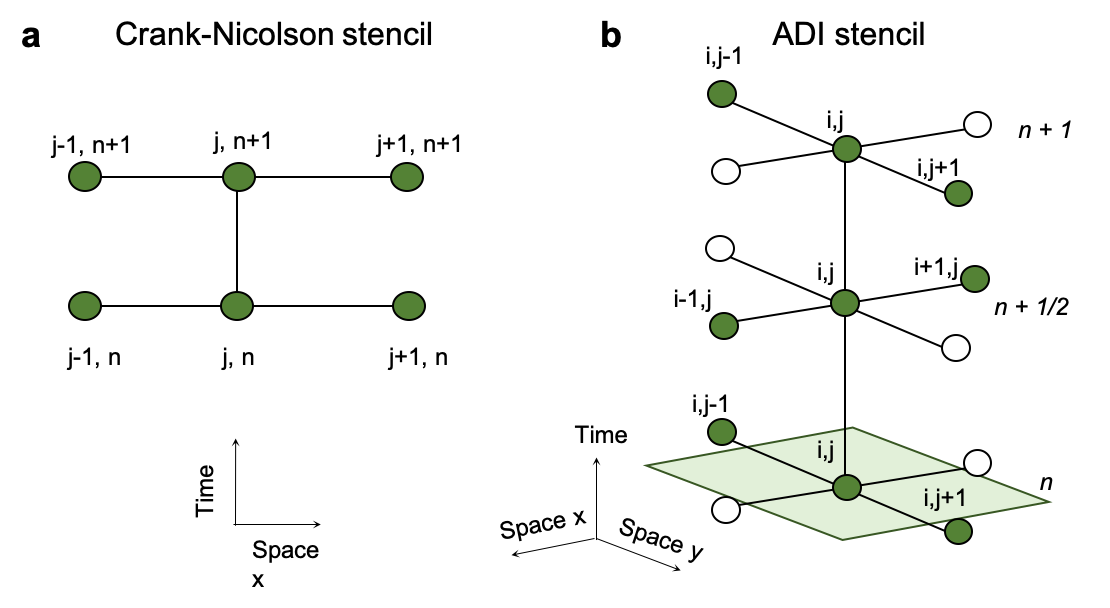
\includegraphics[width=0.8\textwidth,center]{Methods/stencils.png}
%    \caption{\textbf{Stencils for numerical solution}.  A stencil is a geometric representation with nodes and edges, that represents the points of interest for the numerical approximation. The points of interest, which are the ones present in the equations, are shown in green. j and n are the current space and time points. \textbf{(A)} Crank-Nicholson stencil used in 1D numerical simulations. The axis are time and space ($x$). \textbf{(B)} Alternating Direction Implicit method stencil used in 2D numerical simulations. The axis are time and 2 dimensional space ($x$,$y$).}
%\end{figure}
\subsubsection{Crank-Nicolson method}
Consider a reaction diffusion system with one space dimension and boundary conditions
\begin{equation}
    \frac{\delta u}{\delta t} =  f(u) + D\pdv[2]{u}{x},   \quad \quad \quad \quad \quad \quad \pdv{u}{x}\biggr\rvert_{x=0,L}=0
\end{equation}
The spatial part of the equation can be approximated to
\begin{equation}
    \pdv[2]{u}{x} \biggr\rvert_{x=j\Delta x,t=n\Delta t} \approx \frac{1}{2\Delta x^{2}}\left( U^{n}_{j+1} -  2U^{n}_{j} + U^{n}_{j-1} + U^{n+1}_{j+1} - 2U^{n+1}_{j} + U^{n+1}_{j-1}\right),
\end{equation}
while the production function can be approximated to $f ( U^{n}_{j})$.  The approximations can be better visualised using the Crank-Nicolson stencil (See Figure 19a). Applying CN's stencil to the grid point (i,j), the reaction-diffusion system can be expressed as

\begin{equation}
    \frac{U^{n+1}_{j} - U^{n}_{j} }{\Delta t} = \frac{D}{2\Delta x^{2}}\left( U^{n}_{j+1} -  2U^{n}_{j} + U^{n}_{j-1} + U^{n+1}_{j+1} - 2U^{n+1}_{j} + U^{n+1}_{j-1}\right) +  f( U^{n}_{j})
\end{equation}
By reordering this approximation into a linear equation, the resulting problem is defined by a simple linear equation containing matrices A and B. Where $\textbf{U}^{n+1} = [U^{n}_{0}, ... , U^{n}_{J-1}]$, the simplified system can be expressed as:
\begin{equation}
    \textbf{U}^{n+1} = A^{-1}(B\textbf{U}^{n} + f^{n})
\end{equation}
This method simplifies the complex system into a linear system that can be solved numerically. The solution given will be a 1 dimensional in space solution of the reaction-diffusion system. Although the method is  unconditionally stable, the solution can contain oscillations if $ \frac{\Delta t}{\Delta x^{2}} >\frac{1}{2} $ \parencite{trefethen1996finite}. Therefore, the ratio will be kept below $\frac{1}{2}$ to avoid errors.

\subsubsection{Alternating Direction Implicit method}
As done in the CN scheme, a reaction diffusion system and its boundary conditions will be consider. However, in this case two spatial dimensions will be introduced.

\begin{equation}
    \frac{\delta u}{\delta t} =  f(u) + D\left(\pdv[2]{u}{x} + \pdv[2]{u}{y}\right) ,   \quad \quad \quad \quad \quad \quad \pdv{u}{x}\biggr\rvert_{x=0,L}=0 \quad \quad \pdv{u}{y}\biggr\rvert_{y=0,L}=0
\end{equation}
If the CN stencil is applied to this 2 dimensional spatial problem, the system would contain banded matrices in the right and left hand sides, that would be very expensive to invert. ADI offers an alternative in which tridiagonal matrices are inverted instead of banded matrices (less computational power required). The characteristic of ADI is the time step $\Delta t$ is split into two, and each half time step is computed. This means, to compute the change at each time step, first we compute $U^{n+1/2}_{i,j} $ and from there,    $U^{n+1}_{i,j} $ is calculated. This results in two different equations:
\begin{subequations}
    \begin{equation}
        \begin{split}
            \frac{U^{n+1/2}_{i,j} - U^{n}_{i,j} }{\Delta t/2} = \frac{D}{2\Delta x^{2}}\left( U^{n+1/2}_{i+1,j} -  2U^{n+1/2}_{i,j} + U^{n+1/2}_{i-1,j}\right)  \\+ \frac{D}{2\Delta y^{2}}\left( U^{n}_{i,j+1} -  2U^{n}_{i,j} + U^{n}_{i,j-1}\right)  + \Delta t f(U^{n}_{i,j})
        \end{split}
    \end{equation}
    \begin{equation}
        \begin{split}
            \frac{U^{n+1}_{i,j} - U^{n}_{i,j} }{\Delta t/2} = \frac{D}{2\Delta x^{2}}\left( U^{n+1/2}_{i+1,j} -  2U^{n+1/2}_{i,j} + U^{n+1/2}_{i-1,j}\right)  \\+ \frac{D}{2\Delta y^{2}}\left( U^{n+1}_{i,j+1} -  2U^{n+1}_{i,j} + U^{n+1}_{i,j-1}\right)  + \Delta t f(U^{n+1/2}_{i,j})
        \end{split}
    \end{equation}
\end{subequations}
In the first half time step (Equation 46a), the $x$ derivative is taken implicitly, and in the second half time step (Equation 46b), the $y$ derivative is taken implicitly. As done in CN, the approximation is reordered into a linear system. Two families of linear systems appear:
\begin{subequations}
    \begin{equation}
        A\textbf{U}^{n+1/2}_{x,i} = \textbf{b}_{i} + \textbf{f}(\Delta t \textbf{U}^{n}_{x,i}), \quad i=0,...,I-1
    \end{equation}
    \begin{equation}
        C\textbf{U}^{n+1}_{y,j} = \textbf{d}_{j} + \textbf{f}(\Delta t \textbf{U}^{n+1/2}_{y,j}), \quad j=0,...,J-1
    \end{equation}
\end{subequations}
Again, this method also simplifies a complex system into a linear system that can be solved numerically, as in CN. However, this method allows for the introduction of a new spatial dimension and therefore produces a 2D spatial solution. The workings of this method can be better understood with the ADI stencil (See Figure 19b). ADI will be used to visualise patterns in 2D.
\subsubsection{Analysis of numerical solution}
Speed of pattern formation and pattern wavelength are identified by performing additional analysis on the 1D numerical data.  \\\\
\textbf{Time for pattern formation}
The development of the pattern follows a certain behaviour: The molecule concentrations are initially homogeneous; then a pattern gets formed progressively; and finally, the pattern is in its final state and the solution remains constant.  The time for pattern formation is measured by comparing the solution (one point in space) at every time point to the solution at the final time point. If the difference if smaller than a tolerance value of $10^{-4}$ that time point is taken as the convergence time point were the pattern has finished to  develop. \\\\
\textbf{Wavelength prediction from numerical Solution}
The findpeaks package is used from the \textit{scipy.signal} python library. All peaks in the final time point of the 1D simulation are found through the findpeaks package. The average distance between peaks is taken and that distance is averaged throughout the 6 species.

\subsection{Cellular Automata modelling}

\subsection{Machine learning inference of dose response curves}